\section{What is \vampir\ and How is it Used?}

\subsection{Why \vampir?}

\newcommand{\lineOO}{(lO.center) to[out=0, in=180] (sO.center)}
\newcommand{\lineOT}{(lO.center) to[out=-45, in=135] (sT.center)}
\newcommand{\lineOR}{(lO.center) to[out=-80, in=100] (sR.center)}
\newcommand{\lineTO}{(lT.center) to[out=45, in=-135] (sO.center)}
\newcommand{\lineTT}{(lT.center) to[out=0, in=180] (sT.center)}
\newcommand{\lineTR}{(lT.center) to[out=-45, in=135] (sR.center)}
\newcommand{\lineRO}{(lR.center) to[out=80, in=-100] (sO.center)}
\newcommand{\lineRT}{(lR.center) to[out=45, in=-135] (sT.center)}
\newcommand{\lineRR}{(lR.center) to[out=0, in=180] (sR.center)}

\begin{wrapfigure}{r}{0.20\textwidth} %this figure will be at the right
    \centering
    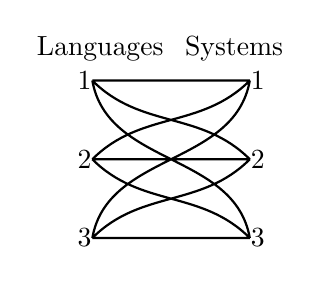
\begin{tikzpicture}
        \node at (1.1, 3.4) {Languages};
        \node (lO) at (1, 3) {};
        \node at (.9, 3) {1};
        \node (lT) at (1, 2) {};
        \node at (.9, 2) {2};
        \node (lR) at (1, 1) {};
        \node at (.9, 1) {3};
        \node at (2.8, 3.4) {Systems};
        \node (sO) at (3, 3) {};
        \node at (3.1, 3){1};
        \node (sT) at (3, 2) {};
        \node at (3.1, 2) {2};
        \node (sR) at (3, 1) {};
        \node at (3.1, 1) {3};
      
      
        \draw[black, thick] \lineOO \lineOT \lineOR \lineTO \lineTT \lineTR \lineRO \lineRT \lineRR;
                
    \end{tikzpicture}
\end{wrapfigure}

\vampir\ is, at its core, a language for defining arithmetic circuits over finite fields. It's intended to be a universal intermediate language supporting many proof systems based on arithmetic circuits. Any higher-level language which intends to compile to arithmetic circuits may target \vampir\ as an intermediate language. 

The need for an intermediate language is obvious. Without an adequate intermediate, systems must support every desired proof system individually. This creates an ecosystem like that depicted in the right figure, where the total work required for interconnectedness is quadratic. This also creates more points of failure and more opportunities for support inconsistencies.

\newcommand{\lineOV}{(lO.center) to[out=-45, in=135] (V.center)}
\newcommand{\lineVO}{(V.center) to[out=45, in=225] (sO.center)}
\newcommand{\lineTV}{(lT.center) to[out=0, in=180] (V.center)}
\newcommand{\lineVT}{(V.center) to[out=0, in=180] (sT.center)}
\newcommand{\lineRV}{(lR.center) to[out=45, in=225] (V.center)}
\newcommand{\lineVR}{(V.center) to[out=-45, in=135] (sR.center)}

\begin{wrapfigure}{l}{0.20\textwidth} %this figure will be at the right
    \centering
    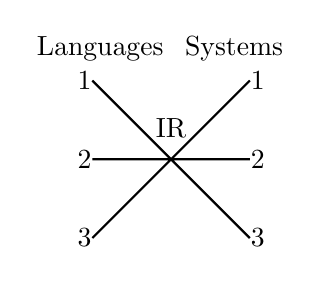
\begin{tikzpicture}
        \node at (2, 2.4) {IR};
        \node (V) at (2, 2) {};
        \node at (1.1, 3.4) {Languages};
        \node (lO) at (1, 3) {};
        \node (lT) at (1, 2) {};
        \node (lR) at (1, 1) {};
        \node at (2.8, 3.4) {Systems};
        \node (sO) at (3, 3) {};
        \node (sT) at (3, 2) {};
        \node (sR) at (3, 1) {};
        
        \node at (.9, 3) {1};
        \node at (.9, 2) {2};
        \node at (.9, 1) {3};
        \node at (3.1, 3){1};
        \node at (3.1, 2) {2};
        \node at (3.1, 1) {3};
      
      
        \draw[black, thick] \lineOV \lineVO \lineTV \lineVT \lineRV \lineVR;
                
    \end{tikzpicture}
\end{wrapfigure}

With an adequate intermediate representation, the total amount of work necessary to fill out the ecosystem is only linear. This can be seen in the ecosystem depicted in the left figure. Languages can, instead of targeting a specific proof system, target the intermediate representation. That language would then have support for every proof system targeted by that intermediate representation.

\vampir's goal is to fulfill this need by providing a minimal and expressive interface for describing the core data structure used by most modern zero-knowledge-proof systems. To that end, \vampir\ aims to be flexible and easy to use but doesn't provide any cryptographic features of its own. It does not presuppose any particular implementation or design for a proof system. \vampir\ files are sufficiently generic that they may even be used for applications that use arithmetic circuits but are not cryptographic in nature.

\subsection{Using \vampir}

A very basic example of a \vampir\ program is the following;

\begin{lstlisting}[language=c]
  // This is a comment!
  def x = 10;

  x = 10;
\end{lstlisting}

Here, one can see the two main top-level commands available in \vampir. That first line defines a constant, \lstinline{x}, to which the value \lstinline{10} is assigned. The second line is an equation that is expected to be true. Every arithmetic circuit is interpreted as a proposition. Specifically, it is the proposition corresponding to the truth of all the equations appearing in the file which generated it. In this case, the compiled circuit will merely check that \lstinline{10 = 10}. Notice that every line must end in a semicolon. \vampir\ does not generally care about white space or newlines (beyond spaces separating individual tokens); this example would be interpreted the same if all newlines were removed and everything was put on a single line.

To compile this circuit, of course, \vampir\ needs to be up and running. First clone \vampir's directory.

\begin{lstlisting}[language=bash]
  $ git clone git@github.com:anoma/vamp-ir
\end{lstlisting}

\vampir\ is implemented in Rust and can easily be compiled from source using Rust Cargo.

\begin{lstlisting}[language=bash]
  $ cd vamp-ir
  $ cargo build
\end{lstlisting}

This will create the \vampir\ binary at `/target/debug/vamp-ir' within the main \vampir\ directory.

\vampir\ does not possess any cryptographic capabilities on its own. This means that some specific parameters, such as the field size, cannot be determined by \vampir, but are instead decided at compile time. To compile this circuit, a target must first be chosen. For this example, I will choose PLONK \textcolor{red}{[What is the name of the program? How does one access other targets?]}.

For the sake of this example, I will assume that the lines in our example program are saved into a file called `ex1.pir', stored within a new folder called `examples' within the main \vampir\ directory. 

\begin{lstlisting}[language=bash]
  $ mkdir examples
  $ printf "def x = 10;\n\nx = 10;">examples/ex1.pir
\end{lstlisting}

Notice the file ends with `.pir', the standard extension for \vampir\ files. To compile this into a PLONK circuit, one must first set up public parameters.

\begin{lstlisting}[language=bash]
  $ target/debug/vamp-ir setup -o examples/params.pp

  > * Setting up public parameters...
  > * Public parameter setup success!
\end{lstlisting}

This will create the file `params.pp' within our `examples' directory. The \lstinline{-o} argument indicates an output file and is equivalent to \lstinline{--output}. One can now create the circuit associated with our file.


\begin{lstlisting}[language=bash]
  $ target/debug/vamp-ir compile -u examples/params.pp \
                                 -s examples/ex1.pir \
                                 -o examples/circuit.plonk

  > * Compiling constraints...
  > ** Inferring types...
  > x[2]: int
  > * Reading public parameters...
  > * Synthesizing arithmetic circuit...
  > * Serializing circuit to storage...
  > * Constraint compilation success!
\end{lstlisting}

This will create our compiled circuit in the file `circuit.plonk' within the `examples' directory. The \lstinline{-u} argument indicates a universal parameter file and is equivalent to \lstinline{--universal-params}. The \lstinline{-s} argument indicates a source file and is equivalent to \lstinline{--source}.

Notice that types for defined expressions are inferred during compilation. \vampir\ has a simple type system that is mostly implicit. This will be explained in more detail later on. In this simple example, \lstinline{x} is inferred to be an `int', that is, an integer that will be interpreted as a field element during compilation.

A zero-knowledge proof of circuit correctness can now be synthesized.

\begin{lstlisting}[language=bash]
  $ target/debug/vamp-ir prove -u examples/params.pp \
                               -c examples/circuit.plonk \
                               -o examples/proof.plonk

  > * Reading arithmetic circuit...
  > * Soliciting circuit witnesses...
  > * Reading public parameters...
  > * Proving knowledge of witnesses...
  > * Serializing proof to storage...
  > * Proof generation success!
\end{lstlisting}

This will create our compiled proof in the file `proof.plonk' within the `examples' directory. The \lstinline{-c} argument indicates a circuit file and is equivalent to \lstinline{--circuit}.

The last thing one may want to do is verify the circuit.

\begin{lstlisting}[language=bash]
  $ target/debug/vamp-ir verify -u examples/params.pp \
                                -c examples/circuit.plonk \
                                -p examples/proof.plonk

  > * Reading arithmetic circuit...
  > * Reading zero-knowledge proof...
  > * Public inputs:
  > * Reading public parameters...
  > * Verifying proof validity...
  > * Zero-knowledge proof is valid
\end{lstlisting}

This will verify the proof just created. In this case, we've just verified a zero-knowledge proof that 10 = 10. The \lstinline{-p} argument indicates a proof file and is equivalent to \lstinline{--proof}. 

Other than \lstinline{help}, every available \vampir\ command has now been used; \lstinline{setup}, \lstinline{compile}, \lstinline{prove}, and \lstinline{verify}. These commands define all current methods for interacting with \vampir. It is a very simple system.

\subsection{Proof Validity and Interaction}

Values for variables do not need to be given upfront. If our file was instead 

\begin{lstlisting}[language=Python, caption={}]
  x = 10;
\end{lstlisting}

without declaring the value of \lstinline{x}, \vampir\ would interpret this unbound variable as an input needing to be specified during proof generation. If this is saved in the file `ex2.pir' and compiled to a circuit, one can see that \vampir\ will ask for an input when it's needed.


\begin{lstlisting}[language=bash]
  $ printf "x = 10;">examples/ex2.pir
  $ target/debug/vamp-ir compile -u examples/params.pp \
                                 -s examples/ex2.pir \
                                 -o examples/circuit2.plonk

  > * Compiling constraints...
  > [...]
  > * Constraint compilation success!

  $ target/debug/vamp-ir prove -u examples/params.pp \
                               -c examples/circuit2.plonk \
                               -o examples/proof2.plonk

  > * Reading arithmetic circuit...
  > * Soliciting circuit witnesses...
  > ** x[2] (private): 
  
  $ 9
  
  > * Reading public parameters...
  > [...]
  > * Proof generation success!
\end{lstlisting}

It asked for the private value for \lstinline{x}, to which I input `9'. This should create an invalid proof this time as 9 does not equal 10. If one tries verifying the proof, they will observe that it's invalid.

\begin{lstlisting}[language=bash]
  $ target/debug/vamp-ir verify -u examples/params.pp \
                                -c examples/circuit2.plonk \
                                -p examples/proof2.plonk

  > * Reading arithmetic circuit...
  > [...]
  > * Verifying proof validity...
  > * Result from verifier: Err(ProofVerificationError)
\end{lstlisting}

As you can see, a verification error is given.